\section{问题一：预热平衡阶段的常物性耦合场模型}

\subsection{模型的具体化}

预热阶段采用附录 2 给出的一组参数，即式~\eqref{eq:app2}：密度、比热容与导热系数取常值，扩散系数只依赖含水率。把它代入公共框架式~\eqref{eq:heat}--\eqref{eq:mass}，热方程的系数不再随解变化，退化为常系数线性方程

\begin{equation}
\frac{\partial T}{\partial t}=\alpha\left(\frac{\partial^2 T}{\partial r^2}+\frac{1}{r}\frac{\partial T}{\partial r}\right),
\qquad
\alpha=\frac{\lambda}{\rho c_p}=\frac{0.36}{820\times2600}=1.6886\times10^{-7}\ \mathrm{m^2/s},
\label{eq:q1alpha}
\end{equation}

水分方程则仍是非线性的，因为扩散系数含 $e^{-0.89/C}$。初始条件按式~\eqref{eq:ic} 取均匀分布。以 $\alpha$ 与初始含水率处的扩散系数 $D(C_0)=4.938\times10^{-9}$~m$^2$/s 分别估算特征时间：热扩散的 $R_0^2/\alpha\approx2.37\times10^3$~s，水分扩散的 $R_0^2/D\approx8.1\times10^4$~s。半小时的观测窗恰好覆盖前者而远短于后者，这就预告了本阶段的基本图景——温度已能贯穿整个截面，水分只在表层附近发生变化。传热毕奥数 ${\rm Bi}_h=1.3889$、初始传质毕奥数 ${\rm Bi}_m=3.2404$，两者都远离集中参数模型的适用范围，径向分布必须保留。

\subsection{求解流程}

本问的求解沿公共框架执行，但因物性为常值而不需要非线性迭代，流程相对简明，如图~\ref{fig:flow-q1}。

\begin{figure}[htbp]
  \centering
  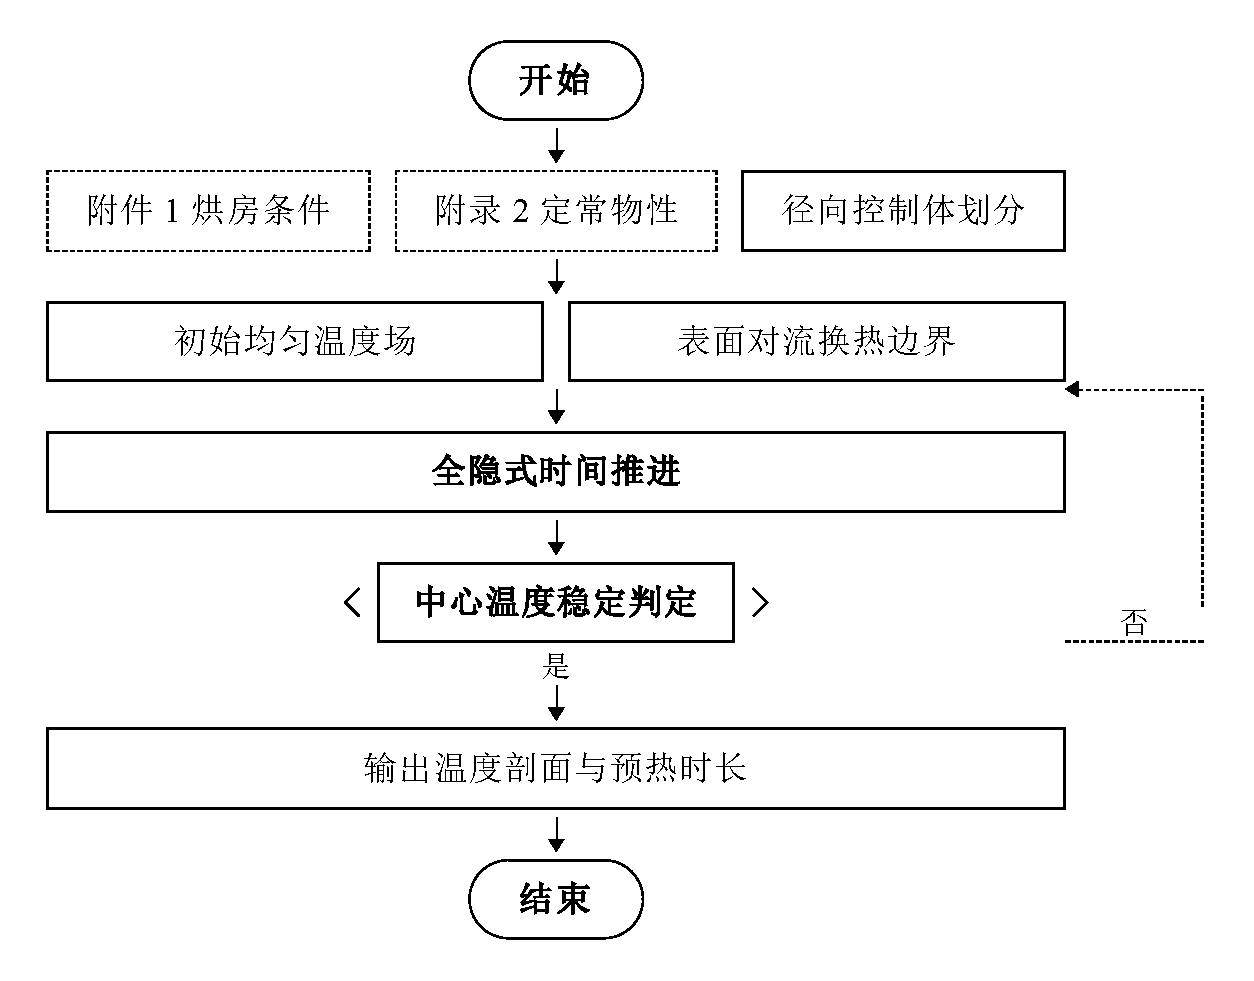
\includegraphics[width=0.8\textwidth,height=0.8\textheight,keepaspectratio]{../figures/fig_flow_q1.pdf}
  \caption{问题 1 的求解流程。自上而下为数据与网格准备、初始与边界设定、全隐式
  时间推进三段，虚线框表示题给数据，加粗框为主控步骤；右侧虚线回路表示中心温度
  未达稳定时返回继续推进，达稳定后输出温度剖面与预热时长。}
  \label{fig:flow-q1}
\end{figure}

流程的三段划分对应三类不同性质的工作：第一段把实测激励和输出网格准备好，网格取 $N=40$ 使节点覆盖全部要求输出的径向位置；第二段把初始条件与两个边界条件装配进系数矩阵；第三段逐步推进并在每步输出。右侧回路的判断依据是中心温度是否仍在明显上升，它决定推进何时终止，而不改变每一步的计算内容。时间步在本问取 $0.01$~s，远小于精度需要，目的是让逐秒输出的结果不受时间离散影响。

\subsection{温度场与水分场的结果}

按题目要求的时刻与位置，温度结果列于表~\ref{tab:q1T}。

\begin{table}[H]
\centering
\caption{30 分钟内药材的温度（单位：°C）}\label{tab:q1T}
\begin{tabular}{cccccc}
\toprule
\multirow{2}{*}{时间/s} & \multicolumn{5}{c}{到药材中心的距离/cm}\\
\cmidrule(lr){2-6}
 & 0 & 0.5 & 1 & 1.5 & 2 \\
\midrule
100  & 28.0001 & 28.0004 & 28.0041 & 28.0327 & 28.1797 \\
300  & 28.0409 & 28.0636 & 28.1514 & 28.3680 & 28.8484 \\
600  & 28.4534 & 28.5361 & 28.8039 & 29.3158 & 30.1649 \\
900  & 29.3244 & 29.4583 & 29.8754 & 30.6160 & 31.7302 \\
1200 & 30.5428 & 30.7098 & 31.2223 & 32.1125 & 33.4275 \\
1500 & 31.9957 & 32.1867 & 32.7660 & 33.7462 & 35.1203 \\
1800 & 33.5753 & 33.7720 & 34.3641 & 35.3621 & 36.7855 \\
\bottomrule
\end{tabular}
\end{table}

表中每一列自上而下都在单调上升，最右列的升幅始终大于最左列，可见升温由表面驱动。同一批时刻与位置上的含水率结果列于表~\ref{tab:q1C}。

\begin{table}[H]
\centering
\caption{30 分钟内药材的水分浓度（单位：kg/kg）}\label{tab:q1C}
\begin{tabular}{cccccc}
\toprule
\multirow{2}{*}{时间/s} & \multicolumn{5}{c}{到药材中心的距离/cm}\\
\cmidrule(lr){2-6}
 & 0 & 0.5 & 1 & 1.5 & 2 \\
\midrule
100  & 2.5500 & 2.5500 & 2.5500 & 2.5500 & 2.2551 \\
300  & 2.5500 & 2.5500 & 2.5500 & 2.5490 & 2.0543 \\
600  & 2.5500 & 2.5500 & 2.5500 & 2.5350 & 1.8788 \\
900  & 2.5500 & 2.5500 & 2.5496 & 2.5044 & 1.7560 \\
1200 & 2.5500 & 2.5500 & 2.5481 & 2.4646 & 1.6595 \\
1500 & 2.5500 & 2.5499 & 2.5444 & 2.4208 & 1.5794 \\
1800 & 2.5500 & 2.5497 & 2.5381 & 2.3757 & 1.5108 \\
\bottomrule
\end{tabular}
\end{table}

两张表呈现出完全不同的节奏。温度方面，半小时内中心由 $28.0000$ 升到 $33.5753$~°C、表面升到 $36.7855$~°C，中心与表面之差始终维持在 $3.2$~°C 左右且各点均在上升，说明热波已经穿透整个截面。含水率方面，表面由 $2.5500$ 降到 $1.5108$~kg/kg，降幅超过四成；而 $r=1$~cm 处仅降到 $2.5381$，中心在四位小数下与初值没有区别。把整个截面平均，含水率由 $2.5500$ 降到 $2.2932$~kg/kg，也就是说这半小时排出的水分几乎全部来自最外侧一层。图~\ref{fig:q1-profiles} 把七个时刻的径向剖面叠在一起。

\begin{figure}[htbp]
  \centering
  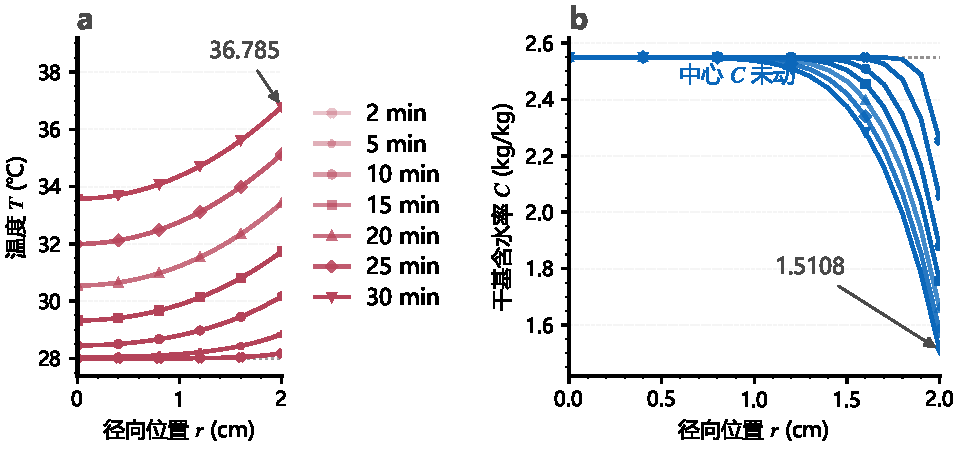
\includegraphics[width=0.9\textwidth,height=0.8\textheight,keepaspectratio]{../figures/fig_q1_profiles.pdf}
  \caption{预热阶段的径向剖面族，7 个输出时刻用同族深浅渐变区分，径向取 21
  个位置（0.1\,cm 间隔）。a：温度剖面自初始均匀态由外向内抬升，表面始终领先
  于中心，中心的追赶速度决定预热时长；b：同期含水率剖面只有表层下降，中心在
  30\,min 内几乎未动，这一快慢分离说明预热段可只看温度判平衡。}
  \label{fig:q1-profiles}
\end{figure}

左图的七条温度剖面整体向上平移而形状变化不大，剖面在表面附近的斜率始终有限，这是第三类边界条件的直接表现：表面温度没有跳到空气温度，而是被对流阻力拖在后面。右图的七条含水率剖面则几乎重合于一条水平线，只在最右端急剧下垂，下垂区宽度约 $0.5$~cm 且随时间缓慢内移。两幅图并置说明，预热阶段判断“是否已经平衡”只需看温度，因为水分场此时尚未真正启动。

把同样的数据换成时间与半径的二维分布，可以更直接地读出两个场的推进速度，见图~\ref{fig:q1-hovmoller}。

\begin{figure}[htbp]
  \centering
  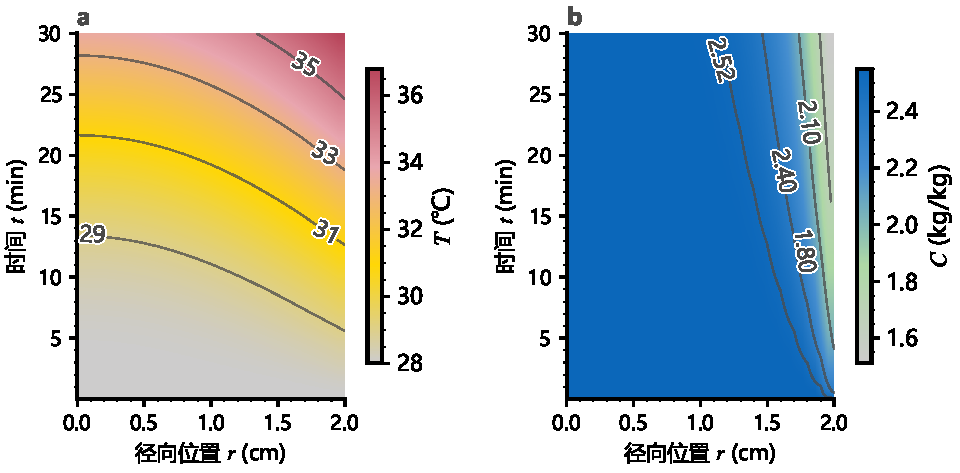
\includegraphics[width=0.9\textwidth,height=0.8\textheight,keepaspectratio]{../figures/fig_q1_hovmoller.pdf}
  \caption{预热阶段温度场与水分场的时间—半径分布（$200\times21$ 输出网格）。
  a：温度等值线自表面向轴线推进，可读出热波到达轴线的时刻与其后的整体抬升；
  b：同期水分场，等值线几乎平行于时间轴，说明 30\,min 内水分尚未形成贯穿性
  梯度。两幅同尺度并置，用于对比热扩散与质扩散的时间尺度差异。}
  \label{fig:q1-hovmoller}
\end{figure}

温度一侧的等值线呈斜向左上的族，每条等值线与纵轴相交的时刻即该温度到达轴线的时刻，可见 $28.5$~°C 的扰动在约 $600$~s 抵达中心，其后各条等值线间距逐渐拉开，反映升温速率随空气温差缩小而放缓。水分一侧的等值线几乎与时间轴平行，全部拥挤在图的右侧边缘，半小时内没有任何一条到达轴线。这两幅图给出的时间尺度比与式~\eqref{eq:q1alpha} 下方由特征时间估算的三十余倍是一致的。

表面通量的演化还揭示了一个不那么直观的现象，见图~\ref{fig:q1-flux}。

\begin{figure}[htbp]
  \centering
  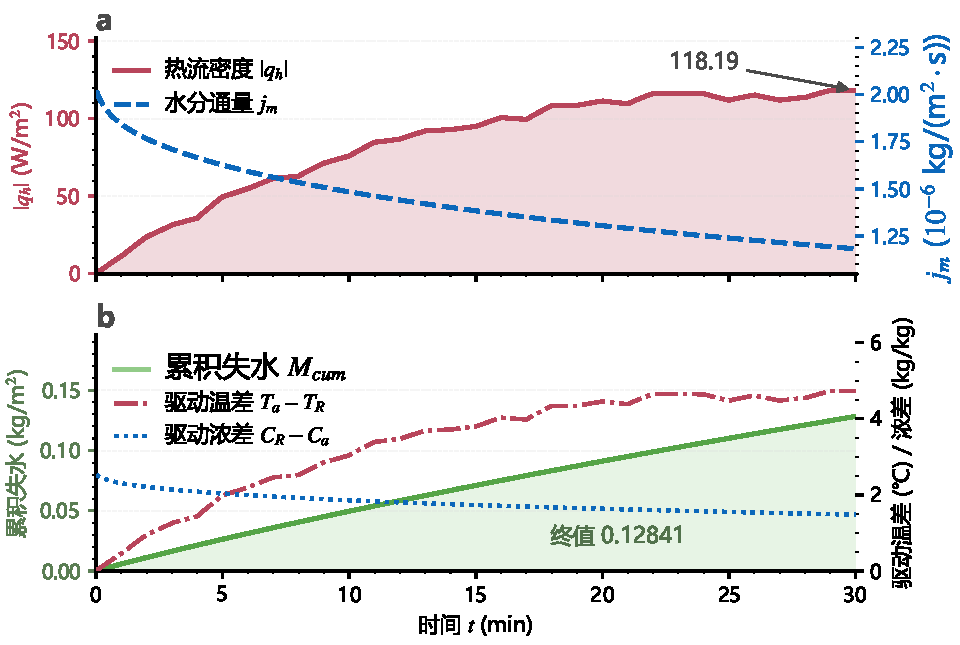
\includegraphics[width=0.9\textwidth,height=0.8\textheight,keepaspectratio]{../figures/fig_q1_flux.pdf}
  \caption{预热阶段表面通量与累积失水（1\,s 输出，1800 点）。a：热流密度
  $|q_h|$ 随表面与空气温差缩小而单调衰减，水分通量 $j_m$ 反而上升，因表面
  升温抬高了平衡含湿的差值；b：累积失水量与两个驱动力（温差、浓差）的同步
  演化，驱动温差衰减而驱动浓差近似持平，故失水近似线性累积。}
  \label{fig:q1-flux}
\end{figure}

热流与水分通量的走向相反：表面热流随着表面温度追近空气温度而单调衰减，水分通量却在同期上升。原因在于两个驱动力的变化方向不同，表面与空气的温差在缩小，而表面含水率与空气水分浓度之差在整个半小时内基本维持，于是累积失水量近似线性增长。这一对照说明预热阶段虽以升温为主，脱水并未停止，只是被限制在表层。表面离散通量与边界条件解析式的残差在全部输出时刻均为零，中心温度始终不超过表面温度，1800 个输出时刻逐一核对无一例外；截面水分的总量平衡残差为 $5.9\times10^{-13}$，处于机器精度量级。
